
\subsection{Introduction \label{introduction}}

Twelve hundred years ago—in a galaxy just across the hill \ldots

First, do not include a title, author block, or \verb|\begin{document}|, etc.
in your paper. We have custom formatting we use for those, and they will be
auto-generated for you during the build process. What you enter into your latex
file will get placed into a template file along with things like your abstract
and keywords. It's very important that you add all of these to your
\texttt{metadata.yaml} file!

Lorem ipsum dolor sit amet, consectetur adipiscing elit. Vestibulum sapien
tortor, bibendum et pretium molestie, dapibus ac ante. Nam odio orci, interdum
sit amet placerat non, molestie sed dui. Pellentesque eu quam ac mauris
tristique sodales. Fusce sodales laoreet nulla, id pellentesque risus convallis
eget. Nam id ante gravida justo eleifend semper vel ut nisi. Phasellus
adipiscing risus quis dui facilisis fermentum. Duis quis sodales neque. Aliquam
ut tellus dolor. Etiam ac elit nec risus lobortis tempus id nec erat. Morbi eu
purus enim. Integer et velit vitae arcu interdum aliquet at eget purus. Integer
quis nisi neque. Morbi ac odio et leo dignissim sodales. Pellentesque nec nibh
nulla. Donec faucibus purus leo. Nullam vel lorem eget enim blandit ultrices.
Ut urna lacus, scelerisque nec pellentesque quis, laoreet eu magna. Quisque ac
justo vitae odio tincidunt tempus at vitae tortor.

\subsection{Bibliographies, citations and block quotes \label{bibliographies-citations-and-block-quotes}}

If you want to include a \texttt{.bib} file, do so above by placing \verb|bibliography: yourFilenameWithoutExtension| in the \texttt{metadata.yaml} file as \verb|yourFilenameWithoutExtension| being sure to remove the \texttt{.bib} extension.

\textbf{Do not include any special characters that need to be escaped or any spaces in the bib-file's name}. Doing so makes bibTeX cranky, \& the rst to LaTeX+bibTeX transform won't work.

To reference citations contained in that bibliography use the \verb|\cite| command, as in \cite{hume48} (which literally is \verb|\cite{hume48}| in accordance with the \texttt{hume48} cite-key in the associated \texttt{mybib.bib} file).

If you wish to have a block quote, use the \verb|\begin{quotation}| and \verb|\begin{quote}| commands, as in:

\begin{quotation}
    \begin{quote}
        When it is asked, What is the nature of all our reasonings concerning matter of fact? the proper answer seems to be, that they are founded on the relation of cause and effect. When again it is asked, What is the foundation of all our reasonings and conclusions concerning that relation? it may be replied in one word, experience. But if we still carry on our sifting humor, and ask, What is the foundation of all conclusions from experience? this implies a new question, which may be of more difficult solution and explication. \cite{hume48}
    \end{quote}
\end{quotation}

\subsubsection{Dois in bibliographies \label{dois-in-bibliographies}}

In order to include a doi in your bibliography, add the doi to your bibliography
entry as a string. For example:
\vspace{1mm}
\begin{verbatim}
    @Book{hume48,
        author = {David Hume},
        year = 1748,
        title = {An enquiry concerning human understanding},
        address = {Indianapolis, IN},
        publisher = {Hackett},
        doi = {10.1017/CBO9780511808432}
    }
\end{verbatim}
\vspace{1mm}

If there are errors when adding it due to non-alphanumeric characters, see if
wrapping the doi in \texttt{\textbackslash{}detokenize} works to solve the issue.

\vspace{1mm}
\begin{verbatim}
    @Book{hume48,
        author = {David Hume},
        year = 1748,
        title = {An enquiry concerning human understanding},
        address = {Indianapolis, IN},
        publisher = {Hackett},
        doi = \detokenize{10.1017/CBO9780511808432},
    }
\end{verbatim}
\vspace{1mm}

\subsection{Citing software and websites \label{citing-software-and-websites}}

Any paper relying on open-source software would surely want to include citations.
Often you can find a citation in BibTeX format via a web search.
Authors of software packages may even publish guidelines on how to cite their work.

For convenience, citations to common packages such as
Jupyter\cite{jupyter},
Matplotlib\cite{matplotlib},
NumPy\cite{numpy},
pandas\cite{pandas1}\cite{pandas2},
scikit-learn\cite{sklearn1}\cite{sklearn2}, and
SciPy\cite{scipy}
are included in this paper's \texttt{.bib} file.

In this paper we not only terraform a desert using the package terradesert\cite{terradesert}, we also catch a sandworm with it.
To cite a website, the following BibTeX format plus any additional tags necessary for specifying the referenced content is recommended.
\vspace{1mm}
\begin{verbatim}
    @Misc{terradesert,
        author = {TerraDesert Team},
        title = {Code for terraforming a desert},
        year = {2000},
        url = {https://terradesert.com/code/},
        note = {Accessed 1 Jan. 2000}
    }
\end{verbatim}
\vspace{1mm}

\subsection{Source code examples \label{source-code-examples}}

Of course, no paper would be complete without some source code.  Without
highlighting, it would look like this:

\begin{verbatim}
    def sum(a, b):
        """Sum two numbers."""

        return a + b
\end{verbatim}

With code-highlighting:

\vspace{1mm}
\begin{Verbatim}[commandchars=\\\{\},fontsize=\footnotesize]
    \PY{k}{def} \PY{n+nf}{sum}\PY{p}{(}\PY{n}{a}\PY{p}{,} \PY{n}{b}\PY{p}{)}\PY{p}{:}
    \PY{+w}{    }\PY{l+s+sd}{\PYZdq{}\PYZdq{}\PYZdq{}Sum two numbers.\PYZdq{}\PYZdq{}\PYZdq{}}

        \PY{k}{return} \PY{n}{a} \PY{o}{+} \PY{n}{b}
\end{Verbatim}
\vspace{1mm}

Maybe also in another language, and with line numbers:

\vspace{1mm}
\begin{Verbatim}[commandchars=\\\{\},numbers=left,firstnumber=1,stepnumber=1,fontsize=\footnotesize,xleftmargin=2.25mm,numbersep=3pt]
    \PY{k+kt}{int}\PY{+w}{ }\PY{n+nf}{main}\PY{p}{(}\PY{p}{)}\PY{+w}{ }\PY{p}{\PYZob{}}
    \PY{+w}{    }\PY{k}{for}\PY{+w}{ }\PY{p}{(}\PY{k+kt}{int}\PY{+w}{ }\PY{n}{i}\PY{+w}{ }\PY{o}{=}\PY{+w}{ }\PY{l+m+mi}{0}\PY{p}{;}\PY{+w}{ }\PY{n}{i}\PY{+w}{ }\PY{o}{\PYZlt{}}\PY{+w}{ }\PY{l+m+mi}{10}\PY{p}{;}\PY{+w}{ }\PY{n}{i}\PY{o}{+}\PY{o}{+}\PY{p}{)}\PY{+w}{ }\PY{p}{\PYZob{}}
    \PY{+w}{        }\PY{c+cm}{/* do something */}
    \PY{+w}{    }\PY{p}{\PYZcb{}}
    \PY{+w}{    }\PY{k}{return}\PY{+w}{ }\PY{l+m+mi}{0}\PY{p}{;}
    \PY{p}{\PYZcb{}}
\end{Verbatim}
\vspace{1mm}

Or a snippet from the above code, starting at the correct line number:
\vspace{1mm}
\begin{Verbatim}[commandchars=\\\{\},numbers=left,firstnumber=2,stepnumber=1,fontsize=\footnotesize,xleftmargin=2.25mm,numbersep=3pt]
    \PY{k}{for}\PY{+w}{ }\PY{p}{(}\PY{k+kt}{int}\PY{+w}{ }\PY{n}{i}\PY{+w}{ }\PY{o}{=}\PY{+w}{ }\PY{l+m+mi}{0}\PY{p}{;}\PY{+w}{ }\PY{n}{i}\PY{+w}{ }\PY{o}{\PYZlt{}}\PY{+w}{ }\PY{l+m+mi}{10}\PY{p}{;}\PY{+w}{ }\PY{n}{i}\PY{o}{+}\PY{o}{+}\PY{p}{)}\PY{+w}{ }\PY{p}{\PYZob{}}
    \PY{+w}{    }\PY{c+cm}{/* do something */}
    \PY{p}{\PYZcb{}}
\end{Verbatim}
\vspace{1mm}


\subsection{Important Part \label{important-part}}

It is well known \cite{Atr03} that Spice grows on the planet Dune.  Test
some maths, for example $e^{\pi i} + 3 \delta$.  Or maybe an
equation on a separate line:

\begin{equation*}
    g(x) = \int_0^\infty f(x) dx
\end{equation*}

or on multiple, aligned lines:

\begin{eqnarray*}
    g(x) &=& \int_0^\infty f(x) dx \\
        &=& \ldots
\end{eqnarray*}

The area of a circle and volume of a sphere are given as

\begin{equation}
    \label{circarea}
    A(r) = \pi r^2.
\end{equation}

\begin{equation}
    \label{spherevol}
    V(r) = \frac{4}{3} \pi r^3
\end{equation}

We can then refer back to Equation (\ref{circarea}) or
(\ref{spherevol}) later.

Mauris purus enim, volutpat non dapibus et, gravida sit amet sapien. In at
consectetur lacus. Praesent orci nulla, blandit eu egestas nec, facilisis vel
lacus. Fusce non ante vitae justo faucibus facilisis. Nam venenatis lacinia
turpis. Donec eu ultrices mauris. Ut pulvinar viverra rhoncus. Vivamus
adipiscing faucibus ligula, in porta orci vehicula in. Suspendisse quis augue
arcu, sit amet accumsan diam. Vestibulum lacinia luctus dui. Aliquam odio arcu,
faucibus non laoreet ac, condimentum eu quam. Quisque et nunc non diam
consequat iaculis ut quis leo. Integer suscipit accumsan ligula. Sed nec eros a
orci aliquam dictum sed ac felis. Suspendisse sit amet dui ut ligula iaculis
sollicitudin vel id velit. Pellentesque hendrerit sapien ac ante facilisis
lacinia. Nunc sit amet sem sem. In tellus metus, elementum vitae tincidunt ac,
volutpat sit amet mauris. Maecenas\footnote{On the one hand, a footnote.} diam
turpis, placerat\footnote{On the other hand, another footnote.} at adipiscing
ac, pulvinar id metus.

\begin{figure}[]
    \noindent
    \makebox[\columnwidth][c]{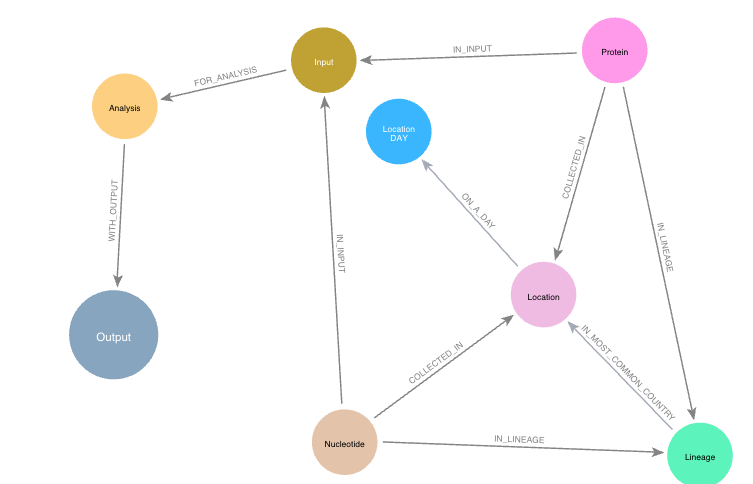
\includegraphics[width=\columnwidth]{figure1.png}}
    \caption{This is the caption. \label{egfig}}
\end{figure}

\begin{figure*}[]
    \noindent
    \makebox[\textwidth][c]{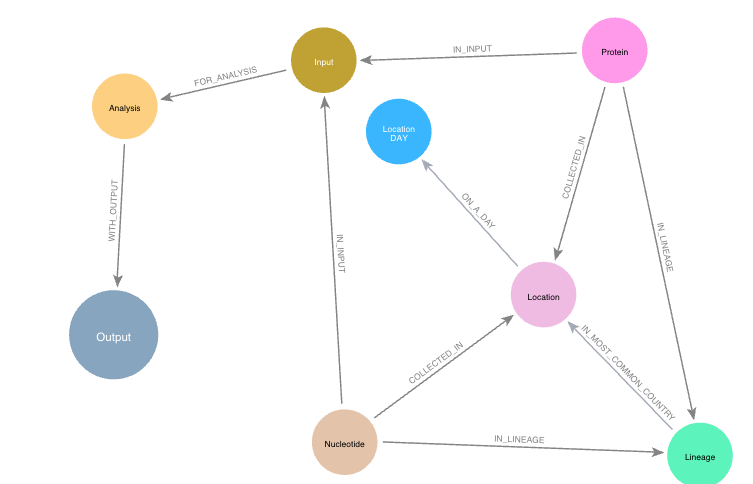
\includegraphics[width=\columnwidth]{figure1.png}}
    \caption{This is a wide figure, specified by adding * to the end of
    the figure environment. It is also center
    aligned, by default}
\end{figure*}

\begin{figure}[bht]
    \noindent
    \makebox[\columnwidth][c]{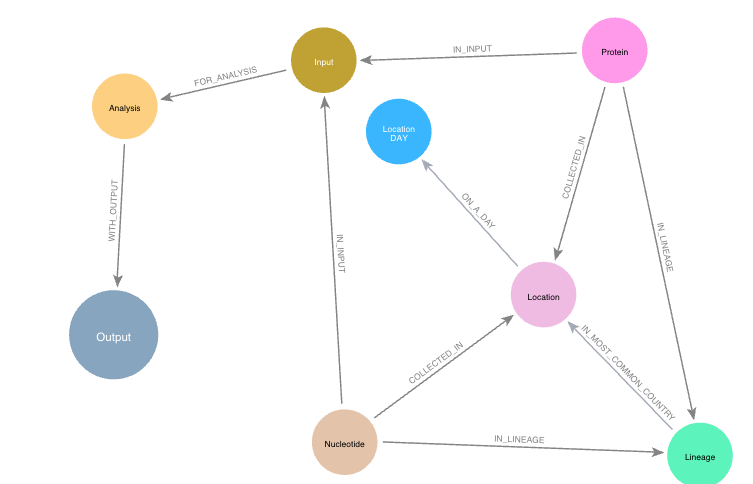
\includegraphics[scale=0.20]{figure1.png}}
    \caption{This is the caption on a smaller figure that will be placed by default at the
    bottom of the page, and failing that it will be placed inline or at the top.
    Note that for now, scale is relative to a completely arbitrary original
    reference size which might be the original size of your image - you probably
    have to play with it. \label{egfig2}}
\end{figure}

As you can see in Figures \ref{egfig} and \ref{egfig2}, this is how you
reference auto-numbered figures.

\begin{table}
    \setlength{\DUtablewidth}{\tablewidth}
    \begin{longtable*}[c]{p{0.156\DUtablewidth}p{0.203\DUtablewidth}}
        \toprule
        \textbf{Material} & \textbf{Units} \\
        \midrule
        \endfirsthead
        Stone & 3 \\
        Water & 12 \\
        Cement & $\alpha$ \\
        \bottomrule
    \end{longtable*}
    \caption{This is the caption for the materials table. \label{mtable}}
\end{table}

We show the different quantities of materials required in Table
\ref{mtable}.

% The statement below shows how to adjust the width of a table.

\setlength{\tablewidth}{0.8\linewidth}
\begin{table*}
    \setlength{\DUtablewidth}{\tablewidth}
    \begin{longtable*}[c]{p{0.110\DUtablewidth}p{0.063\DUtablewidth}p{0.086\DUtablewidth}p{0.086\DUtablewidth}p{0.086\DUtablewidth}p{0.086\DUtablewidth}p{0.110\DUtablewidth}}
        \toprule
        This & is & a & very & very & wide & table \\
        \bottomrule
    \end{longtable*}
    \caption{This is the caption for the wide table.}
\end{table*}

And since you are working in raw latex already, you can easily make complex
table formats. Above we used \verb|\DUtablewidth| to control the width of individual parts of a table, but you can also let tex worry about that part for you:

\begin{table*}
  \begin{longtable*}{|l|r|r|r|}
    \hline
    \multirow{2}{*}{Projection} & \multicolumn{3}{c|}{Area in square miles}\tabularnewline
    \cline{2-4}
    & Large Horizontal Area & Large Vertical Area & Smaller Square Area\tabularnewline
    \hline
    Albers Equal Area  & 7,498.7 & 10,847.3 & 35.8\tabularnewline
    \hline
    Web Mercator & 13,410.0 & 18,271.4 & 63.0\tabularnewline
    \hline
    Difference & 5,911.3 & 7,424.1 & 27.2\tabularnewline
    \hline
    Percent Difference & 44\% & 41\% & 43\%\tabularnewline
    \hline
  \end{longtable*}
  \caption{Area Comparisons \label{quanitities-table}}
\end{table*}

Perhaps we want to end off with a quote by Lao Tse\footnote{$\mathrm{e^{-i\pi}}$}:

\begin{quotation}
    \begin{quote}
        \emph{Muddy water, let stand, becomes clear.}
    \end{quote}
\end{quotation}

